%% ==============================
\chapter{Vergleich der Methoden}
\label{ch:Vergleich}
%% ==============================

In \chapref{ch:Dimensionsreduktion} wurden grundlegende Begriffe geklärt und in
\chapref{ch:MethodenDerDimRed} fünf Methoden der Dimensionsreduktion näher betrachtet. Im jetzigen
Kapitel werden die statistischen Methoden aus \secref{ch:MethodenDerDimRed:statistisch} mit den
Machine Learning Methoden aus \secref{ch:MethodenDerDimRed:modern} empirisch auf künstlichen und
natürlichen Datensätzen verglichen. Dazu wird in \secref{ch:Vergleich:sec:Methodik} auf die
Methodik des Vergleichs eingegangen, indem die Schätzung der intrinsischen Dimension und die
eingesetzten Qualitätskriterien erläutert werden. Außerdem werden in
\secref{ch:Vergleich:sec:VerwendeteDatensaetze} die verwendeten Datensätze und in
\secref{ch:Vergleich:sec:ParameterwahlTrainingsdetails} die Parameterwahl der Methoden vorgestellt.
Letztlich werden in \secref{ch:Vergleich:sec:Resultate} die Resultate des empirischen Vergleichs
diskutiert.

\section{Methodik}
\label{ch:Vergleich:sec:Methodik}

Um die statistischen Methoden mit den Machine Learning Ansätzen zu vergleichen, wird die
Performance der Methoden auf mehreren künstlichen sowie natürlichen Datensätzen mit der
\newterm{Vertrauenswürdigkeit}, der \newterm{Kontinuität} und dem \newterm{Local Continuity
	Meta-Criterion} gemessen. Diese Kriterien werden jeweils für mehrere Nachbarschaftsgrößen
berechnet, um eine größere Aussagekraft über die Güte der gefundenen niedrigdimensionalen
Repräsentation zu erreichen. Die Qualitätskriterien werden in
\subsecref{ch:Vergleich:sec:Methodik:subsec:Qualitaetskriterien} eingehend erläutert. Für den
Vergleich werden zwei künstliche und fünf natürliche Datensätze verwendet, die in
\secref{ch:Vergleich:sec:VerwendeteDatensaetze} genauer vorgestellt werden. Insgesamt soll damit
ein Überblick über die Stärken und Schwächen der statistischen und der Machine Learning Methoden
verschafft werden. Neben dem Vergleich der zwei Gruppen wird in
\secref{ch:Vergleich:sec:Resultate:PCA_AE} der Zusammenhang zwischen der Principal Component
Analysis und Autoencodern genauer untersucht. Der Vergleich kann mittels der im
GitHub-Repository\footnote{\url{www.github.com/MoritzM00/drcomp}} definierten Konfigurationen der
Methoden und des Trainingsskriptes repliziert werden. \rewrite{Unter Methodik könnte man auch was
	anderes verstehen. Ein bisschen mehr dazu sagen, wieso diese Vorgehensweise Sinn macht}

\subsection{Verwendete Qualitätskriterien}
\label{ch:Vergleich:sec:Methodik:subsec:Qualitaetskriterien}
Wie bereits in \chapref{ch:Dimensionsreduktion} erläutert, hat die Dimensionsreduktion das Ziel einer möglichst \enquote{verlustfreien} Transformation der ursprünglichen Repräsentation in eine latente Repräsentation von geringerer Dimension. Für Autoencoder bedeutet \enquote{verlustfrei} die Minimierung des Rekonstruktionsfehlers wie z.B. die quadratische Abweichung (siehe \eqref{eq:MSE_loss}). Dieser Rekonstruktionsfehler ist jedoch wie \textcite[18]{vanderMaaten.2009} hervorhebt, nicht besonders aussagekräftig, da die lokale Struktur der Daten auch mit einem höheren Rekonstruktionsfehler noch erhalten werden kann. Hinzu kommt, dass der Rekonstruktionsfehler nicht für alle Methoden berechenbar ist, da eine inverse Transformation der niedrigdimensionalen in die ursprüngliche Repräsentation benötigt wird. Damit fällt der Rekonstruktionsfehler als geeignetes Qualitätskriterium heraus. Das Forschungsinteresse für Methoden der Dimensionsreduktion hat daher mit der Zeit dafür gesorgt, dass immer mehr Qualitätskriterien entwickelt wurden. \textcite{Gracia.2014} stellen einige Qualitätskriterien vor und vergleichen diese miteinander. Trotzdem gibt es in der Literatur keine eindeutige Kennzahl, die bei einem Vergleich von Dimensionsreduktionsmethoden standardmäßig eingesetzt wird \parencite[vgl.][1 -- 2]{Lee.2009}. Stattdessen bedient man sich mehrerer Kennzahlen, die
unterschiedliche Dinge bestrafen und versucht so die Stärken und Schwächen einer
Dimensionsreduktionsmethode zu erkennen \parencite[486]{Venna.2001}. Die im Folgenden vorgestellten Qualitätskriterien versuchen die Güte
mithilfe von Rängen zu quantifizieren.

Im ausführlichen Benchmark von \textcite{vanderMaaten.2009} wird auf den Generalisierungsfehler
eines 1-Nächste-Nachbar Klassifikators, sowie auf die zwei Kennzahlen Vertrauenswürdigkeit (engl.
\textit{Trustworthiness}) und Kontinuität (engl. \textit{Continuity}) \parencites{Venna.2001}{Venna.2006} gesetzt. Die Vertrauenswürdigkeit und die Kontinuität sind
rangbasierte Qualitätskriterien und werden auch in diesem Vergleich eingesetzt. Daneben gibt es
noch weitere rangbasierte Qualitätskriterien, welche einheitlich durch die sogenannte
\newterm{Co-Ranking-Matrix} \parencite[1432]{Lee.2009} ausgedrückt werden können.\footnote{ Ein Eintrag $q_{kl}$ der Co-Ranking
	Matrix $\mat{Q}$ ist die Anzahl der Paare von Datenpunkten $(i, j)$, die den Rang $r_{\vect{x}}(i,
		j) = k$ in der hochdimensionalen und den Rang $r_{\vect{y}}(i, j) = l$ in der niedrigdimensionalen
	Repräsentation haben. Eine ideale Co-Ranking-Matrix ist eine Diagonalmatrix, da in diesem Fall kein
	Datenpunkt seinen Rang bezüglich eines anderen Punktes geändert hat \parencite[1432]{Lee.2009}. } Ebenso können die im Folgenden betrachteten Qualitätskriterien über die
Co-Ranking-Matrix berechnet werden.

\nomenclature[Z]{LCMC}{Local Continuity Meta-Criterion}

\subsubsection{Vertrauenswürdigkeit und Kontinuität}
\label{ch:Vergleich:sec:Methodik:subsec:Qualitaetskriterien:TC}
Diese beiden Qualitätskriterien basieren auf der Idee des Erhalts von Nachbarschaften (engl.
\textit{neighborhood preservation}) einer Dimensionsreduktion. Sie bilden also ab, wie gut die
lokale Struktur erhalten wird. Formal wird dazu eine $K$-Nachbarschaft $\set{M}_i(K)$ eines Punktes $\vect{x}_i$ als die Menge der Indizes der $K$-nächsten Punkte zu $\vect{x}_i$ mit $i = 1, \ldots, n$ definiert.
Analog kann die $K$-Nachbarschaft $\widetilde{\set{M}}_i(K)$ des dazugehörigen niedrigdimensionalen
Punktes $\vect{y}_i$ definiert werden. Diese Nachbarschaft wird in einer Dimensionsreduktion
erhalten, wenn $\set{M}_i(K) = \widetilde{\set{M}}_i(K)$, das heißt die Nachbarschaften bleiben von
der Dimensionsreduktion unverändert. Zum einen kann es nun passieren, dass weit entfernte Punkte nach der Projektion \textit{nah}
beieinander sind. Mit anderen Worten können Punkte, die eigentlich unterschiedlich sind, nun
ähnlich erscheinen. Aus diesem Grund sagt man, dass die Vertrauenswürdigkeit der
Dimensionsreduktion niedrig ist. Dieser Fall wird über die Menge $\set{U}_i(K)$ formal wie folgt definiert:
\begin{equation}
	\set{U}_i(K) =  \left\{ j \in \N \mid j \notin \set{M}_i(K) \land j \in \widetilde{\set{M}}_i(K) \right\} \, .
\end{equation}

Zum anderen ist der gegenteilige Fall möglich. Nah beieinanderliegende Punkte sind nach der
Projektion weit weg voneinander. Dies reduziert die Kontinuität einer Dimensionsreduktion \parencite[486 -- 487]{Venna.2001} und wird formal über die Menge $\set{V}_i(K)$ als
\begin{equation}
	\set{V}_i(K) =  \left\{ j \in \N \mid j \in \set{M}_i(K) \land j \notin \widetilde{\set{M}}_i(K) \right\}
\end{equation}
definiert. Mithilfe dieser beiden Mengen können nun die beiden Qualitätskriterien wie folgt berechnet werden. Dabei wird die Vertrauenswürdigkeit $T(K)$ über die Menge $\set{U}_i(K)$ mittels
\begin{equation}
	T(K) = 1 - \frac{2}{nK(2n - 3K - 1)} \sum_{i = 1}^{n}\sum_{j \in \set{U}_i(K) } \left( r­_{\vect{y}}(i, j) - K \right)
\end{equation}
berechnet \parencite[487]{Venna.2001}. Hierbei bezeichnet $r_{\vect{y}}(i, j)$ den Rang des niedrigdimensionalen
Vektors $\vect{y}_j$, wenn die Datenpunkte absteigend nach der euklidischen Distanz von
$\vect{y}_i$ geordnet sind. Der Term vor der Summation skaliert das Qualitätskriterium so, dass $0
	\leq T(K) \leq 1$ gilt.\footnote{Dies gilt nur für den Fall, dass $K < n/2$ gilt.} Ein Wert von
$T(K) = 1­$ entspricht einer perfekten Vertrauenswürdigkeit. Eine niedrige Vertrauenswürdigkeit
kann auf ein \enquote{Zusammenziehen} der Mannigfaltigkeit hinweisen, da Punkte nach der
Transformation näher beieinander liegen, als zuvor.

Analog wird die Kontinuität $C(K)$ über $\set{V}_i(K)$ wie folgt definiert
\begin{equation}
	C(K) = 1 - \frac{2}{nK(2n - 3K - 1)} \sum_{i = 1}^{n}\sum_{j \in \set{V}_i(K) } \left( r_{\vect{x}}(i, j) - K \right) \, ,
\end{equation}
wobei $r_{\vect{x}}(i, j)$ nun den Rang zwischen den Datenpunkten in der hochdimensionalen Repräsentation bezeichnet \parencite[487]{Venna.2001}. Auch hier gilt $0 \leq C(K) \leq 1$ und höher ist besser. Die Kontinuität
misst, wie gut die ursprünglichen Nachbarschaften erhalten werden. Eine niedrige Kontinuität kann
darauf hinweisen, dass die Mannigfaltigkeit gezerrt wurde und dadurch die Punkte nach der
Transformation weiter weg voneinander liegen.

Üblicherweise werden die beiden Kriterien für mehrere Werte der Nachbarschaftsgröße $K$ berechnet. So entfällt die willkürliche Wahl einer spezifischen Nachbarschaftsgröße und ermöglicht die Betrachtung von sowohl kleinen als auch größeren Nachbarschaften.

\subsubsection{Local Continuity Meta-Criterion}
\label{ch:Vergleich:sec:Methodik:subsec:Qualitaetskriterien:LCMC}
Das Local Continuity Meta-Criterion (LCMC), entwickelt von \textcite{Chen.2009}, ist ebenso wie die Vertrauenswürdigkeit und Kontinuität ein rangbasiertes Qualitätskriterium. LCMC betrachtet die Überschneidung der $K$-Nachbarschaften in der ursprünglichen und latenten Repräsentation. Nimmt man wieder die $K$-Nachbarschaften als $\set{M}_i(K)$ und $\widetilde{\set{M}}_i(K)$ an, das heißt die Indexmengen der $K$-Nachbarschaften in der ursprünglichen beziehungsweise latenten Repräsentation, dann lässt sich das LCMC wie folgt berechnen \parencite[212]{Chen.2009}:
\begin{equation}
	\label{eq:LCMC}
	\text{LCMC}(K) = \frac{1}{nK} \sum_{i=1}^{n} \left( \left| \set{M}_i(K) \cap \widetilde{\set{M}}_i(K) \right| \right) - \frac{K^2}{n - 1} \,,
\end{equation}
wobei $­|\cdot|$ die Kardinalität einer Menge und $\set{A} \cap \set{B}$ den Durchschnitt zweier Mengen $\set{A}$ und $\set{B}$ bezeichnet. Der Term vor der Summation bildet den Mittelwert und skaliert das Kriterium auf den Wertebereich zwischen Null und Eins, wobei LCMC$(K) = 1$ den besten Wert darstellt. Die Überschneidung der beiden Indexmengen wird wie in \eqref{eq:LCMC} ersichtlich noch um einen additiven Term korrigiert. Dieser Term entspricht dem Erwartungswert einer zufälligen Überschneidung und kann durch eine hypergeometrische Verteilung mit $K$ Defekten aus $n - 1$ bei $K$ Ziehungen modelliert werden \parencite[213]{Chen.2009}. Diese sogenannte Basislinie (engl. \textit{Baseline}) wird mit steigendem
$K$ größer, sodass das Kriterium für den maximalen Wert der Nachbarschaftsgröße $K = n - 1$ den
Wert Null annimmt. Aus diesem Grund besitzt das LCMC ein wohldefiniertes Maximum. Allerdings sind
kleinere Werte von $K$ oftmals wichtiger, um beispielsweise die Erhaltung der Struktur einer
Mannigfaltigkeit zu messen.

\subsection{Schätzen der intrinsischen Dimension}
\label{ch:Vergleich:sec:Methodik:subsec:SchaetzenDerIntrinsischenDim}

Bis jetzt wurde immer angenommen, dass die intrinsische Dimension $d$ der Daten bekannt ist, da die
meisten Dimensionsreduktionsmethoden die intrinsische Dimension nicht selbst berechnen. Das
Schätzen der intrinsischen Dimension ist also ein nicht unwichtiges Teilproblem der
Dimensionsreduktion, da eine Unterschätzung von $d$ dazu führt, dass relevante Strukturen
zwangsweise verloren gehen \parencite[1]{Levina.2004}. Erschwert wird dieses Problem durch die Tatsache, dass es viele
Definitionen der intrinsischen Dimension und damit auch viele unterschiedliche Schätzer gibt. Im
Folgenden soll ein kurzer Überblick verschafft werden, jedoch geht eine detaillierte Behandlung der
Schätzung über den Rahmen dieser Arbeit hinaus. Daher wird für einen Überblick und Vergleich dieser
Schätzer auf \textcites{Campadelli.2015}{Bac.2021}{Verveer.1995} verwiesen.

In \secref{ch:Dimensionsreduktion:MannigfaltigkeitenIntrinsDim} haben wir die \textit{topologische
	Dimension} kennengelernt, welche sich in der Literatur zur Strukturerkennung durchgesetzt hat \parencite[1]{Campadelli.2015}. Allerdings bringt diese Definition praktische Schwierigkeiten mit sich,
weswegen die meisten Schätzer der intrinsischen Dimension auf der damit verwandten
\textit{fraktalen Dimension} wie zum Beispiel der Schätzer der Korrelationsdimension \parencite{Camastra.2002} basieren. Daneben gibt es noch Nächste-Nachbar-basierte Schätzer \parencite[1]{Campadelli.2015}. Zu dieser Kategorie gehört auch der in dieser Arbeit verwendete
\newterm{Maximum Likelihood Schätzer} von \textcite{Levina.2004}. Diese Schätzer betrachten die
Verteilung der Nachbarschaft eines Punktes $\rvect{x}$ als Funktion der intrinsischen Dimension --
üblicherweise innerhalb einer kleinen Kugel um $\rvect{x}$
\parencite[8]{Campadelli.2015}. Der Maximum Likelihood Schätzer nimmt an, dass die Beobachtungen, die
in einer solchen Kugel liegen, einem homogenen Poisson-(Zähl-)Prozess\footnote{Ein
Poisson-Zählprozess ist eine Folge von Zufallsvariablen $\{ N(t) \}_{t \geq 0}$, wobei $N(t) \sim
	\text{Poisson}(\lambda t)$ eine Poisson-verteilte Zufallsvariable ist, die den Wert zum
\textit{Zeitpunkt} $t$ modelliert \parencite[105 -- 117]{Jones.2018}. Dieser Prozess kann dazu benutzt werden, zufällig auftretende
Ereignisse über einen Zeitraum hinweg oder wie hier die Anzahl der Nachbarn eines Punktes zu
zählen.} folgen
\parencite[2]{Levina.2004}.\footnote{Genau genommen, wird zuerst ein inhomogener Binomial-Prozess
	angenommen, der die Punkte mit Distanz kleiner $t$ zählt (bei fixem $\vect{x}$). Dieser Prozess
	wird dann durch einen homogenen Poisson-Prozess approximiert.} Dieser Prozess hängt von $d$ ab,
weshalb mittels der Maximum Likelihood Methode ein Schätzwert $\estNormal{d}$ für einen fixen Punkt
$\rvect{x}_i$ als
\begin{equation}
	\estNormal{d}_K(\vect{x}_i) = \left( \frac{1}{K - 1} \sum_{j=1}^{K - 1} \log \frac{T_K(\vect{x}_i)}{T_j(\vect{x}_i)} \right)^{-1}
\end{equation}
berechnet werden kann \parencite[4]{Levina.2004}. Hierbei ist $K$ die Anzahl der nächste Nachbarn und $T_{K}(\vect{x}_i)$ die
euklidische Distanz von $\vect{x}_i$ zu seinem $K$-ten Nachbar. Dies ist jedoch nur eine lokale
Schätzung für einen fixen Punkt $\vect{x}_i$. Um eine globale Schätzung zu erhalten, wird der
Mittelwert über alle Beobachtungen $\vect{x}_i$ mit $i = 1, \ldots, n$ gebildet.
\section{Verwendete Datensätze}
\label{ch:Vergleich:sec:VerwendeteDatensaetze}
Es werden sowohl künstliche als auch natürliche Datensätze eingesetzt, um Eigenschaften der
verschiedenen Methoden miteinander zu vergleichen. Eine Übersicht über die Dimensionen und Stichprobengrößen der verwendeten Datensätze befindet sich in Tabelle \ref{tab:uebersicht-datensaetze}. Nachfolgend werden zuerst die künstlichen und dann die natürlichen Datensätze beschrieben.

\subsection{Künstliche Datensätze}
\label{ch:Vergleich:sec:VerwendeteDatensaetze:kuenstlich}
Zu den künstlichen Datensätzen gehören die weitverbreitete \textit{Swiss Roll} und der \textit{Twin Peaks} Datensatz,
\begin{figure}[ht]
	\begin{center}
		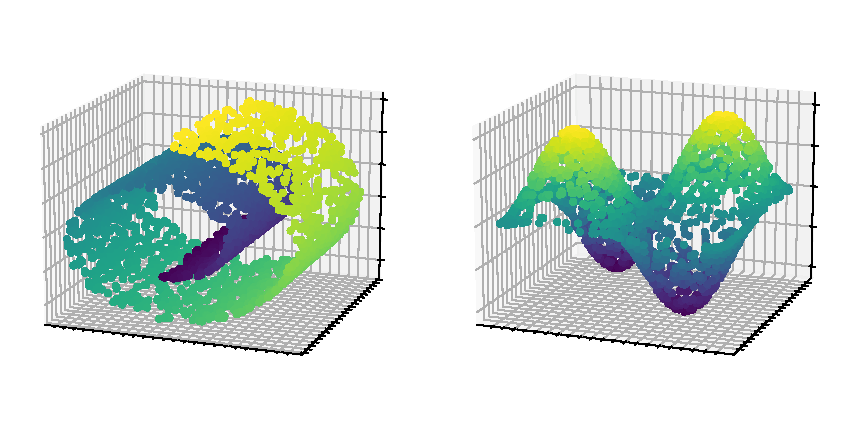
\includegraphics{artificial_datasets.pdf}
	\end{center}
	\caption[Künstliche Datensätze]{\figleft Die Swiss Roll. Die intrinsische Dimension beträgt zwei, da die Daten auf einer \enquote{eingerollten Ebene} liegen. Die Dimensionsreduktionsmethoden müssen die Swiss Roll \enquote{entfalten}, um eine zweidimensionale Repräsentation zu erhalten. \figright Der Twin Peaks Datensatz. Dieser besteht aus vier spitzen Bergen (\textit{Peaks}), wobei je zwei nach oben und unten zeigen. Auch dieser Datensatz hat eine intrinsische Dimension von zwei. Intuitiv gesehen kann man sich lokal nur nach rechts oder links auf der Mannigfaltigkeit bewegen, d.h. die Twin Peaks sind homöomorph zum $\real^2$. Beide 2-Mannigfaltigkeiten sind glatt und zusammenhängend.}
	\label{fig:ArtificialDatasets}
\end{figure}
die in \figref{fig:ArtificialDatasets} dargestellt sind.
Beide künstlichen Datensätze bestehen aus \num{5000} Datenpunkten und haben eine extrinsische Dimension von drei und eine intrinsische
Dimension von zwei. Die Swiss Roll muss von den Dimensionsreduktionsmethoden \enquote{entfaltet} werden, da die Datenpunkte auf einer eingerollten Ebene liegen. Somit könnte die Swiss Roll in einem zweidimensionalen Raum dargestellt werden. Der Twin Peaks-Datensatz besteht aus vier spitzen Bergen, wobei je zwei nach oben und unten zeigen. Die intrinsische Dimension ist auch hier zwei, aber die Dimensionsreduktionsmethoden müssen die Berge sozusagen \enquote{plattdrücken}, um eine zweidimensionale Repräsentation zu erhalten. Der Vorteil einer Evaluierung auf künstlichen Datensätzen ist die visuelle Betrachtung der Datensätze und der gefundenen
latenten Räume der Methoden. Es kann also visuell überprüft werden, ob die Dimensionsreduktionsmethoden eine sinnvolle niedrigdimensionale Repräsentation lernen. Theoretisch könnte dies auch auf natürlichen Datensätzen durchgeführt werden, allerdings ist hier die intrinsische Dimension in der Regel weit über zwei. Bei einer Reduktion auf zwei oder drei Dimensionen würden also zwangsweise Strukturen in den Daten verloren gehen. Künstliche Datensätze sind allerdings nicht zwangsweise aussagekräftig für die Performance auf echten Datensätzen, da diese komplexere Strukturen wie z.B. mehrere nicht-verbundene Untermannigfaltigkeiten aufweisen können. Deswegen wurden zusätzlich fünf natürliche Datensätze zur Evaluierung der Methoden hinzugezogen.

\subsection{Natürliche Datensätze}
\label{ch:Vergleich:sec:VerwendeteDatensaetze:natuerlich}
Im Folgenden werden die im Vergleich eingesetzten natürlichen Datensätze vorgestellt. Es wurden überwiegend Bilddatensätze, aber auch ein Datensatz mit Genausprägungen ausgewählt, da diese eine
hohe extrinsische Dimension aufweisen und daher für die Dimensionsreduktion gut geeignet sind.
Konkret wurden die folgenden Datensätze ausgewählt: (1) \textit{MNIST} \parencite{LeCun.2010}, (2) \textit{Olivetti Research Ltd} (ORL)
\parencite{Samaria.1994}, (3) \textit{Fashion MNIST} \parencite{Xiao.2017}, (4) \textit{Facial Emotion Recognition} (FER) \parencite{DumitruIanGoodfellowWillCukierskiYoshuaBengio.2013} und (5) \textit{Indian Council of
	Medical Research} (ICMR) \parencite{Mohapatra.2022}.

Der weitverbreitete MNIST-Datensatz besteht aus \num{60000} Grauton-Bildern von handgeschriebenen
Zahlen in der Auflösung $28 \times 28$. Die Anzahl der Pixel und damit die
\begin{figure}[h]
	\begin{center}
		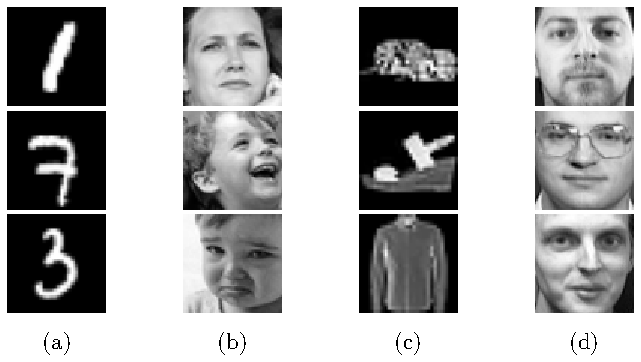
\includegraphics{dataset_samples.pdf}
	\end{center}
	\caption[Beispielbilder der natürlichen Datensätze]{Zu sehen sind Beispielbilder der natürlichen Bilddatensätze aus dem Vergleich: \captiona Handgeschriebene Zahlen aus dem MNIST-Datensatz \captionb Gesichter mit unterschiedlichen Emotionen aus dem FER-Datensatz \captionc Verschiedene Kleidungsstücke aus dem Fashion MNIST-Datensatz \captiond Bilder der Gesichter unterschiedlicher Personen aus zehn Blickwinkeln (ORL-Datensatz)}
	\label{fig:Dataset_samples}
\end{figure}
extrinsische Dimension beträgt 784. Der ORL-Datensatz enthält Bilder von Gesichtern aus
zehn unterschiedlichen Positionen von 40 Personen und ist damit der kleinste natürliche Datensatz
in diesem Vergleich mit 400 Bildern. Die Bilder haben eine Auflösung von $64 \times 64$, was einer
extrinsischen Dimension von \num{4096} entspricht. Der Fashion MNIST-Datensatz besteht aus \num{60000} Bildern
von zehn unterschiedlichen Kleidungsstücken. Die extrinsische Dimension ist ebenso wie bei MNIST
784. Der FER-Datensatz besteht aus \num{28 709} Bildern von Gesichtern mit sieben unterschiedlichen
Emotionen. Die Bilder haben eine Auflösung von $48 \times 48$ und sind damit \num{2304}-dimensional.
Beispiele der Bild-Datensätze sind in \figref{fig:Dataset_samples} zu finden.

\nomenclature[Z]{MNIST}{Modified National Institute of Standards and Technology (Datensatz)}
\nomenclature[Z]{FER}{Facial Emotion Recognition (Datensatz)}
\nomenclature[Z]{ICMR}{Indian Council of Medical Research (Datensatz)}

Letztlich enthält der ICMR-Datensatz Genausprägungen von 801 Personen, die mit fünf
unterschiedlichen Arten von Krebs diagnostiziert wurden. Der Datensatz enthält Genausprägungen von
über \num{20000} Genen, womit dieser Datensatz die höchste extrinsische Dimension im Vergleich
besitzt. In Tabelle \ref{tab:uebersicht-datensaetze} sind die extrinsischen und intrinsischen
Dimensionen, sowie die Stichprobengrößen der Datensätze zusammengefasst. Die intrinsischen
Dimensionen sind die Schätzungen des in
\subsecref{ch:Vergleich:sec:Methodik:subsec:SchaetzenDerIntrinsischenDim} erläuterten Maximum
Likelihood Schätzers für den jeweiligen Datensatz.

\begin{table}[]
	\centering
	\ra{1.3}
	\begin{tabular}{@{}lS[table-format=5.0]S[table-format=2.0]S[table-format=5.0]@{}}
		\toprule
		Datensatz                                 & {$D$} & {$d$} & {$n$} \\ \midrule
		Swiss Roll                                & 3     & 2     & 5000  \\
		Twin Peaks                                & 3     & 2     & 5000  \\
		MNIST                                     & 784   & 15    & 60000 \\
		Fashion MNIST                             & 784   & 18    & 60000 \\
		Indian Council of Medical Research (ICMR) & 20531 & 22    & 801   \\
		Olivetti Research Ltd (ORL)               & 4096  & 9     & 400   \\
		Facial Emotion Recognition (FER)          & 2304  & 26    & 28709 \\
		\bottomrule
	\end{tabular}
	\caption[Übersicht über die extrinsischen und intrinsischen Dimensionen, sowie die Stichprobengrößen der in diesem Vergleich verwendeten Datensätze]{Übersicht über die extrinsischen und intrinsischen Dimensionen, sowie die Stichprobengröße der in diesem Vergleich verwendeten Datensätze. Bei Bilddatensätzen entspricht die extrinsische Dimension der Anzahl der Pixel im Bild. Die intrinsische Dimension wurde mit dem Maximum Likelihood Schätzer aus \subsecref{ch:Vergleich:sec:Methodik:subsec:SchaetzenDerIntrinsischenDim} mit einer Nachbarschaftsgröße $\Kid = 5$ geschätzt.}
	\label{tab:uebersicht-datensaetze}
\end{table}

\section{Trainingsdetails und Parameterwahl}
\label{ch:Vergleich:sec:ParameterwahlTrainingsdetails}

In diesem Abschnitt werden die gewählten (Hyper-)Parameter und Details des Trainierens der
Dimensionsreduktionsmethoden vorgestellt. Eine Übersicht ist in
Tabelle~\ref{tab:uebersicht-parameter} zu finden. Alle Datensätze wurden vor dem Anwenden der
Dimensionsreduktionsmethoden standardisiert, das heißt $\mat{X}$ weist einen spaltenweisen
Erwartungswert von Null und eine spaltenweise Varianz von Eins auf. Für die Evaluierung der
Methoden wurde aufgrund von Restriktionen der Rechenleistung (insbesondere des Arbeitsspeichers)
ein Downsampling auf maximal \num{15000} Stichproben durchgeführt.\footnote{Die Evaluierung ist
	aufgrund der Berechnung der Co-Ranking-Matrix speicherintensiv, da diese maximal $(n-1) \times
		(n-1)$ groß ist und damit quadratisch mit $n$ ansteigt. Um die Qualitätskriterien für den
	MNIST-Datensatz zu berechnen, werden für $n=\num{25000}$ circa 25 GB Arbeitsspeicher benötigt.} Um
die verschiedenen Nachbarschaftsgrößen in Locally Linear Embedding, den Qualitätskriterien und dem
Schätzer der intrinsischen Dimension auseinanderhalten zu können, wird die Notation $\Klle$ für die
Nachbarschaftsgröße in Locally Linear Embedding, $\Kqk$ für die Nachbarschaftsgröße in den
Qualitätskriterien und $\Kid$ für die Nachbarschaftsgröße des Schätzers der intrinsischen Dimension
für den restlichen Teil dieser Arbeit eingeführt.

Für die Principal Component Analysis gibt es neben der Anzahl der zu behaltenden Hauptkomponenten
keine Parameter. Die Anzahl der Hauptkomponenten entspricht der intrinsischen Dimension, welche vom
Datensatz abhängt und für alle Methoden identisch ist. Dies trifft analog auf Kernel PCA und auf
Locally Linear Embedding zu. Für Autoencoder bestimmt die intrinsische Dimension die Größe der
Bottleneck-Schicht. Für Kernel PCA wird ein Gaußscher Kernel eingesetzt, wofür ein Hyperparameter
$\sigma$ gewählt werden kann. Die Werte $\sigma \in \{ 0.1, 0.25, 0.75, 1, 2, 5\}$ wurden getestet
und der beste Durchlauf ausgewählt. Für ICMR und ORL lieferten diese Werte schlechte Ergebnisse,
weswegen auf diesen Datensätzen zusätzlich die Werte \numlist{e-5;e-4;e-3;e-2;e-1} getestet wurden.
Für Locally Linear Embedding gibt es nur einen Parameter $\Klle$, der die Größe der verwendeten
Nachbarschaft kontrolliert. Die Werte $\Klle \in \{ 5, 7, 10, 12, 15\}$ wurden getestet und der
beste Durchlauf ausgewählt.

Den statistischen Methoden gegenüber haben Autoencoder deutlich mehr Freiheitsgrade, um die
Architektur zu bestimmen. Die wichtigsten Parameter sind die Anzahl der Schichten $m$, sowie die
Anzahl an Neuronen pro Schicht und die Wahl der Aktivierungsfunktionen. Daneben gibt es noch viele
weitere Freiheitsgrade beim Trainieren des Autoencoders, welche teilweise vom Datensatz abhängen.
Die Architekturen und weitere Trainingsdetails werden in
Appendix~\ref{ch:Appendix:Architektur-Details} genauer erläutert. Auf Bilddatensätzen wurden
zusätzlich Convolutional Autoencoder trainiert, deren Architekturen an \textcite[14]{Ghosh.2019}
angelehnt und ebenfalls in Appendix~\ref{ch:Appendix:Architektur-Details} spezifiziert sind.

\begin{table}[ht]
	\tymax=300pt
	\centering
	\ra{1.3}
	\begin{tabulary}{\linewidth}{LC}
		\toprule
		Methode                            & Parameter                                                            \\ \midrule
		PCA      & --                                                                   \\
		Kernel PCA                         & $\kappa(\vect{x}_1, \vect{x}_2) = \exp(- \norm{\vect{x}_1 - \vect{x}_2}^2/(2\sigma))$, $\sigma \in \{\num{e-5},\num{e-4}, \num{e-3}, \num{e-2}, \num{e-1}, 0.25, 0.75, 1, 2, 5\}$ \\
		Locally Linear Embedding     & $\Klle \in \{ 5, 7, 10, 12, 15\}$,                      \\
		Autoencoder                  & $m \in \{3, 5, 7\}$, Sigmoid-Aktivierungsfunktion \newline (siehe
		Appendix~\ref{ch:Appendix:Architektur-Details})                                                           \\  Contractive Autoencoder & $m \in \{3, 5\}$, $\lambda=1\mathrm{e}{-4}$,
		Sigmoid-Aktivierungsfunktion (siehe Appendix~\ref{ch:Appendix:Architektur-Details})                       \\
		Convolutional Autoencoder & $m > 5$, ReLU-Aktivierungsfunktion \newline (siehe
		Appendix~\ref{ch:Appendix:Architektur-Details})                                                           \\ \bottomrule
	\end{tabulary}
	\caption[Übersicht über die verwendeten Parameter der Methoden]{Übersicht über die verwendeten Parameter. Hierbei ist $\kappa$ die Kernel-Funktion, $\Klle$ die Nachbarschaftsgröße, $m$ die Anzahl der Schichten im Autoencoder und $\lambda$ eine multiplikative Konstante für den kontrahierenden Fehlerterm des CAE.}
	\label{tab:uebersicht-parameter}
\end{table}
\section{Resultate}
\label{ch:Vergleich:sec:Resultate}

In diesem Abschnitt werden die Resultate des empirischen Vergleichs vorgestellt. Die verschiedenen
Methoden wurden mit den im vorhergehenden \secref{ch:Vergleich:sec:ParameterwahlTrainingsdetails}
erläuterten Parametern auf den künstlichen und natürlichen Datensätzen trainiert\footnote{Die
	einzelnen Durchläufe wurden mittels \textit{Weights \& Biases} aufgezeichnet und sind im
	\textit{drcomp}-Projekt zu finden
	(\url{https://wandb.ai/moritzm00/drcomp?workspace=user-moritzm00}).} und hinsichtlich der in
\secref{ch:Vergleich:sec:Methodik:subsec:Qualitaetskriterien} vorgestellten Qualitätskriterien für
eine Nachbarschaftsgröße von $1 \leq \Kqk \leq 100$ evaluiert. In
\secref{ch:Vergleich:sec:Resultate:kuenstlich} werden die Ergebnisse auf den künstlichen
Datensätzen und in \secref{ch:Vergleich:sec:Resultate:natuerlich} die Ergebnisse auf den
natürlichen Datensätzen diskutiert. Letztlich wird in \secref{ch:Vergleich:sec:Resultate:PCA_AE}
der Zusammenhang zwischen der Principal Component Analysis und Autoencodern empirisch untersucht.

\subsection{Resultate auf künstlichen Datensätzen}
\label{ch:Vergleich:sec:Resultate:kuenstlich}

Zuerst werden die Resultate auf den beiden künstlichen Datensätzen diskutiert. Dabei sind in
\figref{fig:SwissRollMetrics} die drei Qualitätskriterien für die Swiss Roll und im Appendix in
\figref{fig:TwinPeaksMetrics} für den Twin Peaks-Datensatz abgebildet.
\begin{figure}[ht]
	\begin{center}
		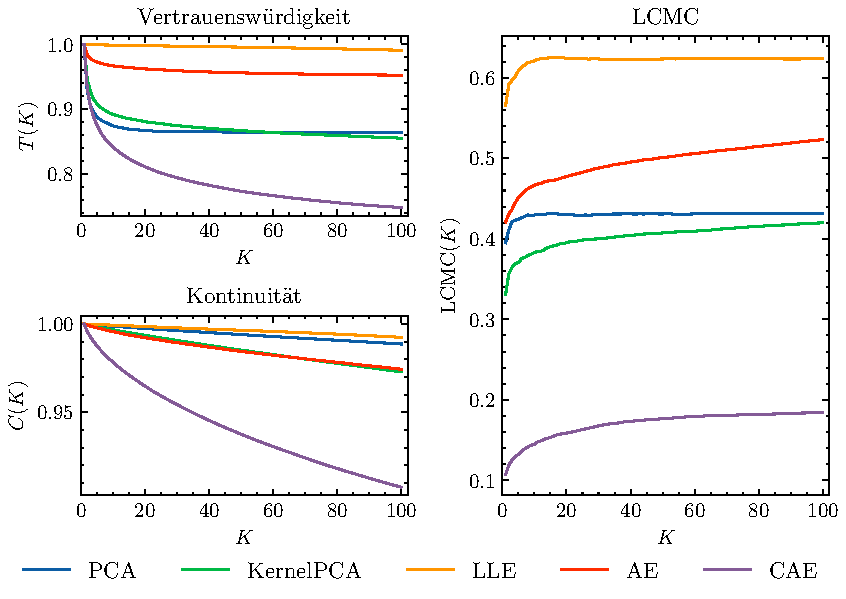
\includegraphics{SwissRoll_comparison.pdf}
	\end{center}
	\caption[Qualitätskriterien für die Swiss Roll]{Die Vertrauenswürdigkeit und Kontinuität der Dimensionsreduktion, sowie das Local Continuity Meta-Criterion (LCMC) für den Swiss Roll Datensatz. Locally Linear Embedding (LLE) schneidet mit Abstand am besten ab, gefolgt vom klassischen Autoencoder. Die restlichen Methoden fallen insbesondere hinsichtlich der Vertrauenswürdigkeit und des LCMC nach unten ab. Der Autoencoder zeigt hier den Vorteil durch die Flexibilität in der Architektur gegenüber der linearen Principal Component Analysis, welche mehr Schwierigkeiten mit dieser nichtlinearen Mannigfaltigkeit hat. (Eigene Darstellung)}
	\label{fig:SwissRollMetrics}
\end{figure}
Beide Abbildungen zeigen ein ähnliches Ergebnis: Locally Linear Embedding kann mit der lokalen Erhaltung der Struktur hohe Werte auf allen drei Qualitätskriterien erzielen. Insbesondere hinsichtlich des LCMC kann sich LLE deutlich nach oben absetzen.
Der Autoencoder zeigt auf dem Swiss Roll-Datensatz die zweithöchste Vertrauenswürdigkeit. PCA, Kernel PCA und der Contractive Autoencoder sind hier deutlich weniger vertrauenswürdig. Bei diesen Methoden werden also nach der Dimensionsreduktion mehr Punkte fälschlicherweise Nachbarn. Auf dem Twin Peaks-Datensatz schneidet neben dem Autoencoder auch die Kernel PCA besser ab. Etwas deutlicher fällt hier die Principal Component Analysis zurück. Diese Methode hat Schwierigkeiten mit dem hohen Grad an Nichtlinearität in den beiden künstlichen Datensätzen. Der Contractive Autoencoder schneidet auf allen drei Kriterien relativ gesehen am schlechtesten ab. Möglicherweise verhindert der kontrahierende Fehlerterm die Anpassung an die Mannigfaltigkeit mit einer hohen Krümmung wie im Twin Peaks-Datensatz.

Die Ergebnisse auf den künstlichen Datensätzen können visuell überprüft werden, indem die
zweidimensionalen transformierten Daten $\mat{Y}$ in einem Scatter-Plot dargestellt werden. Diese
Möglichkeit der Visualisierung der latenten Repräsentation ist ein Vorteil der Evaluierung auf
künstlichen Datensätzen. Dies könnte theoretisch auch auf den natürlichen Datensätzen durchgeführt
werden, allerdings gehen dabei zwangsweise Strukturen verloren, da die intrinsische Dimension auf
diesen Datensätzen weit über zwei liegt. Als Illustration wurden in
\figref{fig:SwissRollEmbeddings}
\begin{figure}[ht]
	\centering
	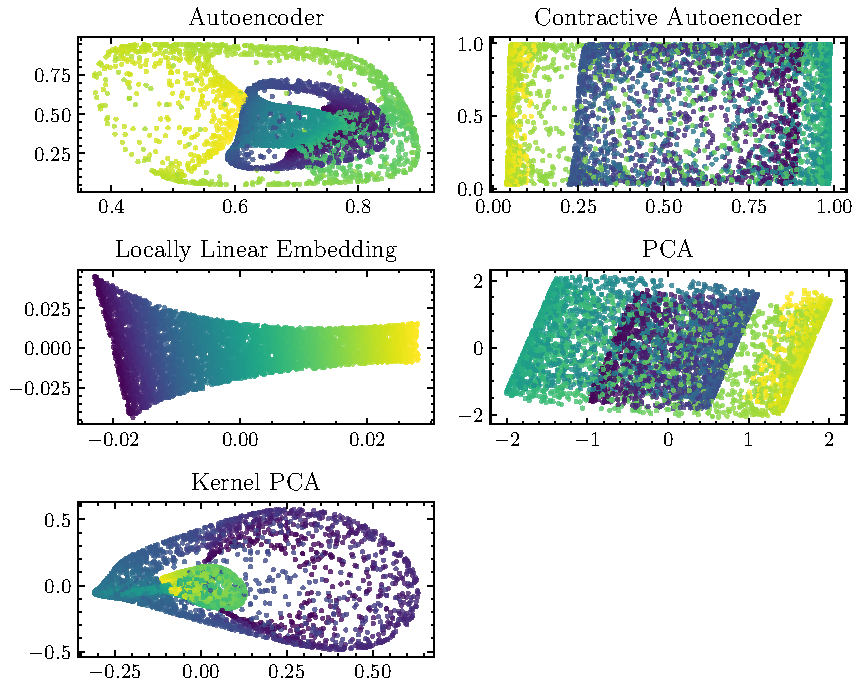
\includegraphics{SwissRollEmbeddings.pdf}
	\caption[Latente zweidimensionale Repräsentationen  $\mat{Y}$ durch Anwendung fünf unterschiedlicher Methoden auf dem Swiss Roll-Datensatzes]{Abgebildet sind die latenten zweidimensionalen Repräsentationen $\mat{Y}$ durch Anwendung fünf unterschiedlicher Methoden auf dem Swiss Roll-Datensatz. Nur Locally Linear Embedding ist in der Lage, die Swiss Roll zu \enquote{entfalten}. Dies ist angesichts der hohen Qualitätskriterien von Locally Linear Embedding und der niedrigeren Qualitätskriterien der restlichen Methoden auf diesem Datensatz stimmig (siehe \figref{fig:SwissRollMetrics}). (Eigene Darstellung)}
	\label{fig:SwissRollEmbeddings}
\end{figure}
die latenten Repräsentationen $\mat{Y} \in \real^{n \times 2}$ durch Anwendung der fünf Methoden auf den Swiss Roll-Datensatz in einem Scatter-Plot dargestellt.
% Dasselbe Vorgehen wurde auch auf dem Twin Peaks-Datensatz durchgeführt und ist in
% \figref{fig:TwinPeaksEmbeddings} zu finden. 
Locally Linear Embedding ist als einzige Methode in der Lage, die Swiss Roll zu
\enquote{entfalten}. Dies bestätigt die hohe Vertrauenswürdigkeit und Kontinuität der
Dimensionsreduktion durch Locally Linear Embedding und die niedrigeren Werte der restlichen
Methoden (siehe \figref{fig:SwissRollMetrics}). Die niedrigere Vertrauenswürdigkeit hat
insbesondere für die Visualisierung eine große Bedeutung, da dies anzeigt, dass Punkte in der
latenten Repräsentation Nachbarn werden, obwohl sie es ursprünglich nicht waren. Nur der
Autoencoder kann ebenfalls eine höhere Vertrauenswürdigkeit erzielen, da die Swiss Roll teilweise
entfaltet werden kann. Die inneren Punkte werden allerdings näher zueinander gezerrt, was die
Kontinuität dieser Dimensionsreduktion reduziert. Sowohl die klassische Principal Component
Analysis, als auch die Kernel-Variante sind nicht in der Lage, die Swiss Roll zu entfalten.

\subsection{Resultate auf natürlichen Datensätzen}
\label{ch:Vergleich:sec:Resultate:natuerlich}

Die Qualitätskriterien auf den natürlichen Datensätzen zeigen ein etwas anderes Bild, als es bei
den künstlichen Datensätzen der Fall war. Die guten Ergebnisse von Locally Linear Embedding setzen
sich nicht auf den natürlichen hochdimensionalen Datensätzen fort.
\begin{figure}[ht]
	\begin{center}
		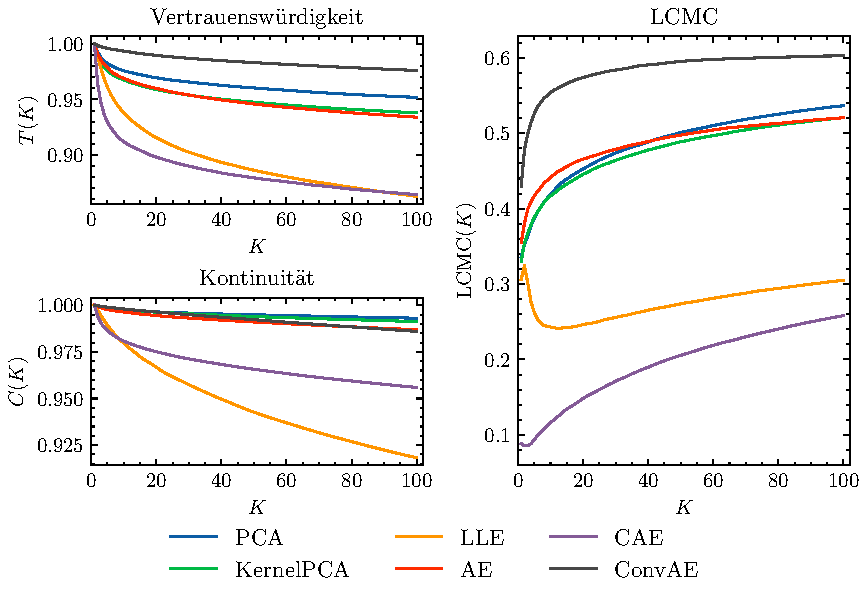
\includegraphics{MNIST_comparison.pdf}
	\end{center}
	\caption[Qualitätskriterien für MNIST]{Die Vertrauenswürdigkeit und Kontinuität der Dimensionsreduktion, sowie das Local Continuity Meta-Criterion (LCMC) für den MNIST-Datensatz. Auf diesem Datensatz kann der der domänenspezifische Convolutional Autoencoder (ConvAE) seine Stärken zeigen, da der Datensatz von hoher Qualität ist und viele Trainingsdaten zur Verfügung stehen. Principal Component Analysis, sowie Kernel PCA und der klassische Autoencoder schneiden ähnlich ab, d.h. die Nichtlinearität der letzteren beiden Methoden kann hier keine nennenswerte Verbesserungen hervorbringen. Locally Linear Embedding und der Contractive Autoencoder können auf allen drei Qualitätskriterien nicht mit den anderen Methoden mithalten. (Eigene Darstellung)}
	\label{fig:MNISTMetrics}
\end{figure}
Auf allen natürlichen Datensätzen
schneidet Locally Linear Embedding hinsichtlich aller drei Kriterien neben dem Contractive Autoencoder relativ gesehen schlecht ab. Insbesondere nehmen die
Qualitätskriterien von Locally Linear Embedding mit größer werdender Nachbarschaftsgröße $\Kqk$ deutlicher ab, als bei den
restlichen Methoden. Der Parameter $\Klle$ für Locally Linear Embedding wurde jedoch auf kleinere Werte zwischen fünf und 15 gesetzt, weswegen diese Beobachtung logisch erscheint. Die Principal Component Analysis kann auf fast allen natürlichen Datensätzen eine gute oder sogar die
beste relative Performance aufweisen. Ebenso zeigt die Kernel PCA gute Ergebnisse und ist auf dem ICMR- und ORL-Datensatz fast identisch zur klassischen Principal Component Analysis. Der klassische Autoencoder kann die Principal Component Analysis auf den Qualitätskriterien nicht mehr übertreffen. Auf den vier Bilddatensätzen kann jedoch der Convolutional
Autoencoder seine Stärken zeigen, allerdings nur, wenn genügend Trainingsdaten zur Verfügung stehen. Letzteres trifft unter anderem auf den MNIST-Datensatz zu, nicht jedoch auf den ORL-Datensatz. Auf diesem Datensatz ist das Ergebnis nur minimal besser, als das des klassischen Autoencoders. Im direkten Vergleich zur Principal Component Analysis schneidet der Convolutional Autoencoder hier aber schlechter ab.
Auf Datensätzen mit einer geringen Anzahl an Stichproben können Probleme bei der Konvergenz der iterativen Optimierung eines Autoencoders auftreten. Dies wird durch die Performance des vollvernetzten Autoencoders auf dem ORL-Datensatz ersichtlich (siehe \figref{fig:OlivettiFacesMetrics}). Insbesondere hinsichtlich des LCMC fällt der Autoencoder nach unten ab. Dies ist ein Nachteil einer iterativen Optimierung der Zielfunktion gegenüber einer Lösung in geschlossener Form.

Die Resultate auf den Bilddatensätzen zeigen jedoch, dass der Convolutional Autoencoder eine valide
Alternative zum klassischen Autoencoder ist, falls Bilddaten oder ähnliches in der Dimension
reduziert werden sollen und genug Trainingsdaten vorhanden sind. Allerdings muss dabei, wie im
Folgenden ersichtlich wird, eine höhere Laufzeit in Kauf genommen werden.

\subsubsection{Vergleich der Laufzeiten}

Nicht zu vernachlässigen ist der zeitliche Aufwand, den die Methoden auf den Datensätzen benötigen.
Dazu sind in \tabref{tab:training_times} die Laufzeiten aller Methoden für alle Datensätze
aufgelistet.

\def\sym#1{\ifmmode^{#1}\else\(^{#1}\)\fi}
\begin{table}[ht]
	\centering
	\ra{1.3}
	\resizebox{\textwidth}{!}{
		\begin{tabular}{l*7{S[table-align-text-post=false]}}
			\toprule
			\multirow{2}[2]{*}{Methode} & \multicolumn{7}{c}{Laufzeit in Sekunden}                                                                                                                        \\
			\cmidrule{2-8}              & {MNIST}                                  & {Fashion MNIST}  & {Twin Peaks}    & {Swiss Roll}     & {ORL}           & {ICMR}          & {FER}                    \\
			\midrule
			PCA                         & 2,00                                     & 2,54             & 0,01            & 0,00             & 0,35            & 0,78            & 2,51                     \\
			Kernel PCA                  & 101,00\sym{*}                            & 101,72\sym{*}    & 0,62            & 0,59             & 0,03            & 1,01            & 103,17\sym{*}            \\
			LLE                         & 417,41\sym{**}                           & 447,95\sym{**}   & 0,45            & 0,42             & 0,24            & 1,14            & \bfseries 426,50\sym{**} \\
			AE                          & 161,35                                   & 121,14           & \bfseries 45,32 & \bfseries 102,34 & 43,02           & 54,51           & 102,26                   \\
			CAE                         & 403,74                                   & 641,00           & 30,04           & 22,68            & 5,76            & \bfseries 93,06 & 361,72                   \\
			ConvAE                      & \bfseries 467,61                         & \bfseries 754,83 & {--}            & {--}             & \bfseries 50,20 & {--}            & 249,64                   \\
			\bottomrule
			\multicolumn{8}{l}{\footnotesize Hinweis: Die Berechnung erfolgte auf einer zufällig gezogenen Teilmenge der Größe (\sym{*}) \num{15000} bzw. (\sym{**}) \num{20000}}                         \\
		\end{tabular}
	}
	\caption[Laufzeiten der Dimensionsreduktionsmethoden in Sekunden.]{Laufzeiten der einzelnen Dimensionsreduktionsmethoden in Sekunden (niedriger ist besser). Alle statistischen Methoden wurden auf einer Intel Xeon Gold 5315Y CPU mit \num{3,20} GHz Taktfrequenz und alle Machine Learning Methoden auf einer NVIDIA RTX A4000 Grafikkarte trainiert. Die höchsten Werte pro Datensatz wurden fett markiert. PCA weist auf allen Datensätzen, inklusive der etwas größeren Datensätze MNIST und Fashion MNIST, eine kurze Laufzeit von maximal \num{2,5} Sekunden auf. Die Laufzeiten der anderen beiden statistischen Methoden Kernel PCA und LLE steigen bei Datensätzen mit einer höheren Stichprobengröße stark an. Die längsten Laufzeiten weisen der Convolutional und Contractive Autoencoder auf.}
	\label{tab:training_times}
\end{table}

Die Principal Component Analysis weist die durchschnittlich geringste Laufzeit auf und untermauert die bereits guten Ergebnisse auf den Qualitätskriterien. Die Laufzeiten von Locally Linear Embedding sind auf kleineren Datensätzen noch kurz, steigen aber mit der Stichprobengröße stark an. Gleiches trifft auf Kernel Principal Component Analysis zu. Der Grund dafür ist, dass Locally Linear Embedding ein dünn besetztes Eigenwertproblem der $n \times n$-Matrix $\mat{M}$ (\eqref{eq:LLE:ZielfunktionY}) lösen muss. Die Laufzeit dieser Operation steigt quadratisch mit $n$ an, was für große Stichproben schnell kostspielig wird \parencite[9]{Saul.2000}. Locally Linear Embedding wurde aus diesem Grund mit maximal \num{20000}
Stichproben trainiert. Bei Kernel PCA musste aufgrund der Eigenwertzerlegung der $n \times
	n$-Kernel-Matrix ebenfalls ein Downsampling durchgeführt werden, falls die Stichprobengröße
\num{15000} übersteigt.

Die höchste Laufzeit weist der Convolutional Autoencoder auf dem Fashion MNIST-Datensatz mit 755
Sekunden oder circa 13 Minuten auf. Der Contractive Autoencoder hat ebenfalls auf den größeren
Datensätzen eine hohe Laufzeit. Dies ist unter anderem der allgemeinen Implementierung des
kontrahierenden Fehlerterms geschuldet. Eine spezifische Implementierung wie in
\eqref{eq:CAE-loss-simple} könnte die Laufzeiten des Contractive Autoencoders noch verbessern,
schränkt dafür aber die Architektur in diesem Fall auf dreischichtige Autoencoder mit
Sigmoid-Aktivierungsfunktionen ein.

Das manuelle Hyperparameter-Tuning wurde hierbei nicht berücksichtigt. Dies ist ein weiterer
Vorteil der Principal Component Analysis, da es hier keine Parameter gibt, die richtig eingestellt
werden müssen. Insbesondere bei der Kernel PCA müssen mehrere Werte für den Parameter $\sigma$
getestet werden. Aufgrund der relativ niedrigen Laufzeiten der Kernel PCA ist dies jedoch
vertretbar. Der Zeitaufwand für Hyperparameter-Tuning ist bei Autoencodern wegen der vielen zu
wählenden Parameter höher. Bei einem Einsatz dieser Methode in der Dimensionsreduktion muss daher
mit einem hohen Zeitaufwand für manuelles oder automatisiertes Hyperparameter-Tuning gerechnet
werden. Dies ist ein entscheidender Nachteil der hier vorgestellten Machine Learning Ansätze.
Allerdings wird das Hyperparameter-Tuning auch für Kernel PCA und Locally Linear Embedding auf
größeren Datensätzen teuer.

\subsubsection{Vergleich der Rekonstruktionen}

Interessant ist außerdem, wie gut die Dimensionsreduktionsmethoden ein originales Bild wieder
rekonstruieren können. In diesem Vergleich können allerdings nur die Principal Component Analysis
und alle Varianten der Autoencoder für die Rekonstruktion verwendet werden. Kernel PCA und Locally
Linear Embedding erlauben ohne Approximation keine inverse Transformation aus der latenten
Repräsentation $\vect{y}$ zurück in eine approximierte ursprüngliche Repräsentation
$\estNormal{\vect{x}}$. Für die Principal Component Analysis, den vollvernetzten Autoencoder, den
Convolutional Autoencoder und für den Contractive Autoencoder wurde auf dem MNIST-Datensatz je ein
Beispielbild für eine der Zahlen rekonstruiert und in \figref{fig:MNIST-reconstructions}
abgebildet. Die erste Zeile besteht aus den Originalbildern als Referenz.
\begin{figure}[ht]
	\centering
	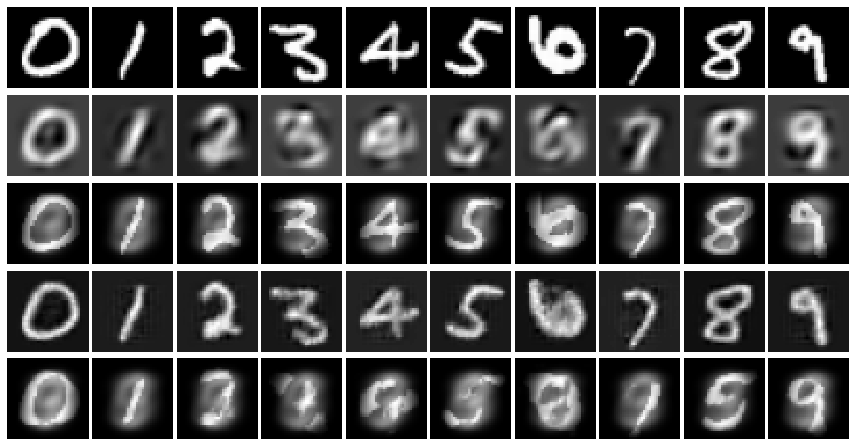
\includegraphics{reconstructions_mnist_pca_ae_convae_cae.pdf}
	\caption[Rekonstruierte MNIST-Zahlen]{Gezeigt sind rekonstruierten Zahlen aus dem MNIST-Datensatz von mehreren Methoden. Jede Zeile gehört zu einer Methode. Von oben nach unten: (1) Originale Bilder als Referenz, (2) Rekonstruktion durch PCA, (3) Rekonstruktion durch einen vollvernetzten Autoencoder, (4) Rekonstruktion durch den Convolutional Autoencoder und (5) Rekonstruktion durch den Contractive Autoencoder.}
	\label{fig:MNIST-reconstructions}
\end{figure}
Visuell ist die beste Rekonstruktion die des Convolutional Autoencoders, gefolgt vom vollvernetzten Autoencoder. Insbesondere die Rekonstruktionen des Contractive Autoencoders sind nicht gut, da einige Zahlen sogar als falsche Zahl rekonstruiert werden. Die Rekonstruktionen der Principal Component Analysis sind besser, aber visuell ebenfalls nicht überzeugend, da sie deutlich unscharfer sind. Der hier eingesetzte tiefe Convolutional Autoencoder mit mehr als 10 Schichten hat über zwölf Millionen trainierbare Gewichte und zeigt auf dem MNIST-Datensatz hinsichtlich der Qualitätskriterien eine gute Güte der Dimensionsreduktion (siehe \figref{fig:MNISTMetrics}). Allerdings ist MNIST ein relativ simpler Datensatz von hoher Qualität, sodass dieser tiefe Autoencoder scheinbar eine sinnvolle Repräsentation lernen kann. Beispielsweise ist der FER-Datensatz deutlich komplexer als MNIST mit einer geringeren Anzahl an Trainingsdaten. Auf diesen Datensätzen ist die Rekonstruktion des Convolutional Autoencoders nicht mehr so gut wie auf dem MNIST-Datensatz.

\subsection{Principal Component Analysis vs. Autoencoder}
\label{ch:Vergleich:sec:Resultate:PCA_AE}

In diesem Abschnitt wird die Principal Component Analysis mit Autoencodern verglichen. Dazu wird
der theoretische Zusammenhang zwischen den beiden Methoden erklärt und durch empirische Experimente
verdeutlicht.

\subsubsection{Theoretischer Zusammenhang}

\textcites{Baldi.1989}{Bourlard.1988} haben gezeigt, dass die Kodierung $\vect{y} = f(\vect{x})$ eines linearen Autoencoders äquivalent -- aber nicht identisch -- zu den Hauptkomponenten $\tr{\mat{A}}\vect{x}$ einer Principal Component Analysis ist. Im Falle eines dreischichtigen Autoencoders sind, wie bereits in \eqref{eq:dreischichtigerAE} erklärt wurde, die Gewichte des Encoders eine Matrix $\mat{W}_1 \in \real^{d \times D}$ und die Gewichte des
Decoders eine Matrix $\mat{W}_2 \in \real^{D \times d}$. Für den Rest dieses Abschnitts werden daher ausschließlich dreischichtige Autoencoder betrachtet. Es kann nun gezeigt werden, dass sich die Zielfunktion eines solchen Autoencoders mit linearen Aktivierungsfunktionen (LAE) auf die Form
\begin{equation}
	\mathcal{J}_{\text{LAE}} = \norm{\mat{X} - \mat{W}_2\mat{W}_1\mat{X}}_F^2
\end{equation}
reduziert \parencite[292]{Bourlard.1988}. Das Eckhart-Young-Mirsky-Theorem \parencite{Eckart.1936} sagt nun aus, dass das optimale $\mat{W} = \mat{W}_2 \mat{W}_1$ auf die
Eigenvektorbasis der Kovarianzmatrix von $\mat{X}$ projiziert \parencite[vgl.][1]{Kunin.2019}. Ein linearer Autoencoder ohne Regularisierung der Gewichte
(\textit{weight decay}) lernt allerdings nur einen Unterraum davon, da diese Zielfunktion durch
eine invertierbare Matrix $\mat{G}$ äquivalent umformuliert werden kann zu \parencite[1]{Kunin.2019}
\begin{equation}
	\mathcal{J}_{\text{LAE}} = \norm{\mat{X} - (\mat{W}_2\mat{G}^{-1}) (\mat{G} \mat{W}_1)\mat{X}}_F^2 \, .
\end{equation}
Die Gewichte eines linearen Autoencoders, der den quadrierten Fehler
(\eqref{eq:AE_objectiveFunction}) minimiert, spannen also einen äquivalenten Unterraum wie
Ladungsmatrix $\mat{A}$ auf. Dies gilt sogar dann, wenn im Encoder Sigmoid-Aktivierungsfunktionen verwendet werden \parencite[291, 293]{Bourlard.1988}. Jedoch unterscheidet sich die latente Repräsentation $\mat{Y}$
eines linearen Autoencoders mit der von PCA wie folgt \parencite[3]{Plaut.2018}: (1) Die Kovarianzmatrix von $\mat{Y}$ ist nicht diagonal, das heißt die
latente Repräsentation ist nicht unkorreliert.\footnote{Äquivalent dazu ist die Korrelationsmatrix
	von $\mat{Y}$, welche lediglich eine skalierte Kovarianzmatrix darstellt, keine Einheitsmatrix.}
(2) Die Spalten von $\mat{Y}$ sind nicht nach absteigender Varianz sortiert. (3) Hat man einen
Encoder $f: \real^D \rightarrow \real^{k_1}$ und möchte man einen Vektor $\vect{x} \in \real^D$ auf
nur $k_2$ Dimensionen mit $k_2 < k_1$ reduzieren, so können nicht einfach die ersten $k_2$
Koordinaten von $f(\vect{x})$ verwendet werden. Das bedeutet, dass die Lösungen von Autoencodern
auf unterschiedliche Dimensionen nicht geschachtelt sind.

Es wurden jedoch bereits Verfahren entwickelt, mit denen diese Eigenschaften wiederhergestellt oder
von Beginn an sichergestellt werden können. Das Vorgehen von \textcite{Plaut.2018} rekonstruiert
mittels eines linearen Autoencoders die Eigenvektorbasis der Kovarianzmatrix bis hin zu einer
orthogonalen Transformation. Die Autoren behaupten, dass durch eine Singulärwertzerlegung der
Decoder-Gewichtsmatrix $\mat{W}_2$, d.h. die Zerlegung in
\begin{equation}
	\label{eq:SVD}
	\mat{W}_2 = \mat{U} \mat{\Psi} \tr{\mat{V}}
\end{equation}
die Hauptkomponenten bis hin zu einer orthogonalen Transformation erlangt werden können \parencite[4]{Plaut.2018}.\footnote{Die Singulärwertzerlegung ist eine Verallgemeinerung der
	Eigenwertzerlegung für nicht-quadratische Matrizen, wie es hier mit $\mat{W}_2 \in \real^{D \times
			d}$ der Fall ist. $\mat{U}$ und $\mat{V}$ sind orthogonale Matrizen, die aus den Links-
	beziehungsweise Rechts-Singulärvektoren bestehen. Die Matrix $\mat{\Psi}$ ist eine Diagonalmatrix
	mit den Singulärwerten \parencite[44 -- 45]{Goodfellow.2016}. } Dabei sind die ersten $d$ Links-Singulärvektoren, d.h. die
ersten $d$ Spalten von $\mat{U}$, die gesuchten Vektoren. Allerdings wurde dies nicht formal
bewiesen, sondern nur in empirischen Ergebnissen festgestellt. Eine Re-Implementierung des
beschriebenen Vorgehens schlägt fehl, wenn ein linearer Autoencoder ohne \textit{weight decay}
verwendet wird. Diese Beobachtung wurde in der Arbeit von \textcite{Kunin.2019} zur Landschaft der
Fehlerfunktion eines linearen Autoencoders bestätigt und formal nachgewiesen. Damit ein linearer
Autoencoder die Richtungen der Hauptkomponenten lernen kann, muss ein Regularisierungsterm zur
Zielfunktion des Autoencoders hinzufügt werden, der die Größe der Gewichte bestraft (siehe
Regularisierung in \secref{ch:MethodenDerDimRed:ML:AE}).

\subsubsection{Visualisierung der Zusammenhänge}

Der eben beschriebene Zusammenhang wird im Folgenden zur Verdeutlichung visualisiert. Dazu wird
zuerst die Korrelation der transformierten Daten und anschließend werden die gefundenen Gewichte
der Methoden genauer analysiert. Punkt (1) aus dem theoretischen Zusammenhang wird in
\figref{fig:Kovarianzmatrizen} deutlich.
\begin{figure}[ht]
	\centering
	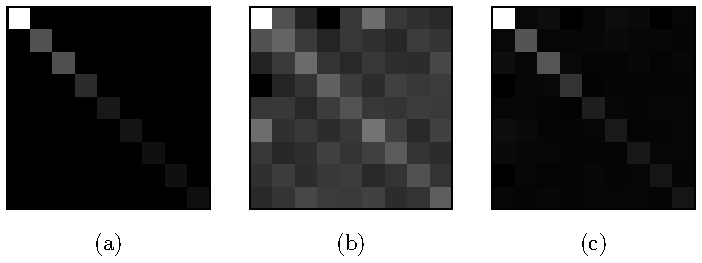
\includegraphics{covariance-matrices.pdf}
	\caption[Kovarianzmatrizen der transformierten Daten $\mat{Y}$ für den FER-Datensatz von drei Methoden]{Die Kovarianzmatrizen der transformierten Daten $\mat{Y}$ für den FER-Datensatz, wobei in \captiona die Principal Component Analysis und die Links-Singulärvektoren der Decoder-Gewichtsmatrix eines linearen Autoencoders \captionb ohne \textit{weight decay} und \captionc mit \textit{weight decay} verwendet wurde, um die Daten auf neun Dimensionen zu reduzieren. Die Kovarianzmatrix bei Transformation mittels der Principal Component Analysis ist per Konstruktion eine Diagonalmatrix mit absteigend sortierten Varianzen, das heißt es besteht keine Korrelation in $\mat{Y}$. Wendet man die Singulärwertzerlegung auf die Decoder-Gewichtsmatrix des linearen Autoencoders an, so erhält man ohne \textit{weight decay} keine Diagonalmatrix. Wurde hingegen \textit{weight decay} verwendet, so ist die Kovarianzmatrix eine Diagonalmatrix. (Eigene Darstellung, angelehnt an \textcite[5]{Plaut.2018})}
	\label{fig:Kovarianzmatrizen}
\end{figure} Dargestellt sind die Kovarianzmatrizen der transformierten Daten, wobei in \captiona die Principal Component Analysis und jeweils die Links-Singulärvektoren der Decoder-Gewichtsmatrix eines linearen Autoencoders \captionb ohne \textit{weight decay} und \captionc mit \textit{weight decay} verwendet wurde, um die Daten auf neun Dimensionen zu reduzieren. Die Kovarianzmatrix bei der Principal Component Analysis ist wie erwartet eine Diagonalmatrix mit absteigend sortieren Varianzen auf der Diagonalen. Die von \textcite{Plaut.2018} vorgeschlagene Methode wurde in \captionb und \captionc angewandt. Hierbei bestimmt jedoch die Verwendung von \textit{weight decay} die Orthogonalität der latenten Repräsentation. Wird keine Regularisierung verwendet, so besteht Korrelation in $\mat{Y}$. Im Gegensatz dazu konnte die Korrelation fast vollständig eliminiert werden, wenn \textit{weight decay} verwendet wird.

Um nun die gefundenen Lösungen einer Principal Component Analysis und von Autoencodern genauer
betrachten zu können, kann die Ladungsmatrix $\mat{A}$ mit den Gewichtsmatrizen eines Autoencoders
verglichen werden. Auf Bilddatensätzen können diese Matrizen so umgeformt werden, dass sich für
jede Zeile von $\mat{W}_1$ oder Spalte von $\mat{W}_2$ ein Bild ergibt.
\figref{fig:Gewichtsvergleich} setzt dieses Vorgehen auf dem FER-Datensatz um.
\begin{figure}[ht]
	\centering
	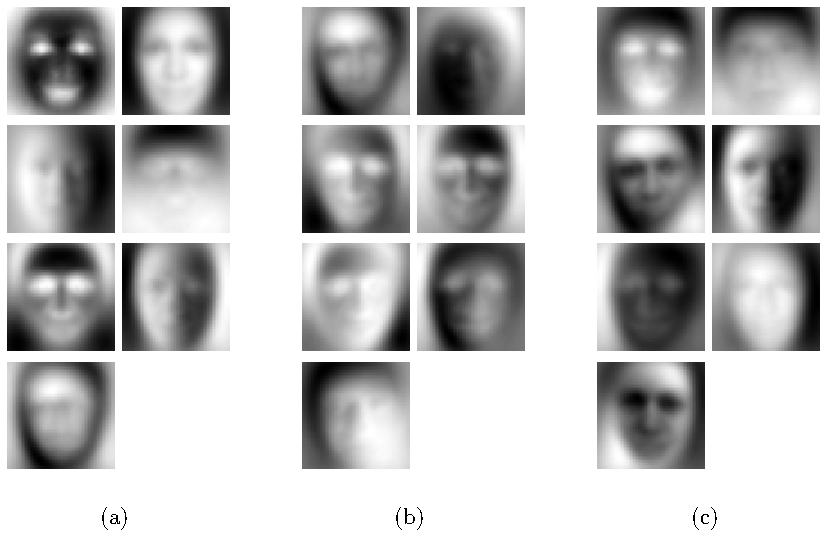
\includegraphics{weights-comparison.pdf}
	\caption[Die Gewichtsmatrizen von drei Methoden auf dem FER-Datensatz]{Gezeigt sind die Gewichtsmatrizen von drei Methoden bei einer Reduktion des FER-Datensatzes auf neun Dimensionen. Ein einzelnes Bild entspricht einer Spalte der Ladungs- beziehungsweise Gewichtsmatrix, welche in die Größe des Bildes umgeformt wurde. \captiona Die Ladungsmatrix $\mat{A}$ der Principal Component Analysis. \captionb Die Decoder-Gewichtsmatrix eines linearen Autoencoders ohne \textit{weight decay}. \captionc Die Links-Singulärvektoren der Decoder-Gewichtsmatrix eines linearen Autoencoders \captionb mit \textit{weight decay}. (Eigene Darstellung, angelehnt an \textcite[5]{Plaut.2018})}
	\label{fig:Gewichtsvergleich}
\end{figure}
Hierbei sind in \figref{fig:Gewichtsvergleich} \captiona die Ladungsmatrix von PCA, in \captionb die Decoder-Gewichtsmatrix eines linearen Autoencoders und in \captionc die ersten $d$ Links-Singulärvektoren der Decoder-Gewichtsmatrix eines linearen Autoencoders mit \textit{weight decay} dargestellt.
Die Gewichte des linearen Autoencoders zeigen bereits eine Ähnlichkeit zu der Ladungsmatrix $\mat{A}$ der Principal Component Analysis, jedoch sind einige Unterschiede erkennbar. Die Links-Singulärvektoren der Decoder-Gewichtsmatrix sind bis auf das Vorzeichen fast identisch zur Ladungsmatrix $\mat{A}$.

Zusammenfassend bedeutet dies, dass ein dreischichtiger Autoencoder mit linearen
Aktivierungsfunktionen eine ähnliche latente Repräsentation wie die Principal Component Analysis
lernt. Eine Regularisierung der Gewichte begünstigt dabei Orthogonalität in der gefundenen Lösung
des Autoencoders. Damit kann für sehr große Datensätze ein alternativer Algorithmus mithilfe des
Autoencoders verwendet werden, um die Richtungen der Hauptkomponenten zu lernen. Dabei umgeht man
die Eigenwertzerlegung der $D \times D$-Kovarianzmatrix der Daten, indem nur die
Singulärwertzerlegung der $D \times d$-Gewichtsmatrix $\mat{W}_2$ berechnet werden muss.

\subsubsection{Hinzunahme von Nichtlinearität}

Im Folgenden wird untersucht, inwiefern die Hinzunahme von Nichtlinearität die latente
Repräsentation eines Autoencoders beeinflusst. Dazu wurden mehrere dreischichtige Autoencoder mit
unterschiedlichen Aktivierungsfunktionen auf dem MNIST-Datensatz trainiert, wobei schrittweise
Nichtlinearität hinzugefügt wird. Mithilfe dieser Autoencoder wurde dann die latente Repräsentation
$\mat{Y}$ für den MNIST-Datensatz berechnet und in \figref{fig:Autoencoder-Nichtlinearitaet}
dargestellt. Für Visualisierungszwecke wurde die intrinsische Dimension dabei auf zwei gesetzt.
\begin{figure}[ht]
	\centering
	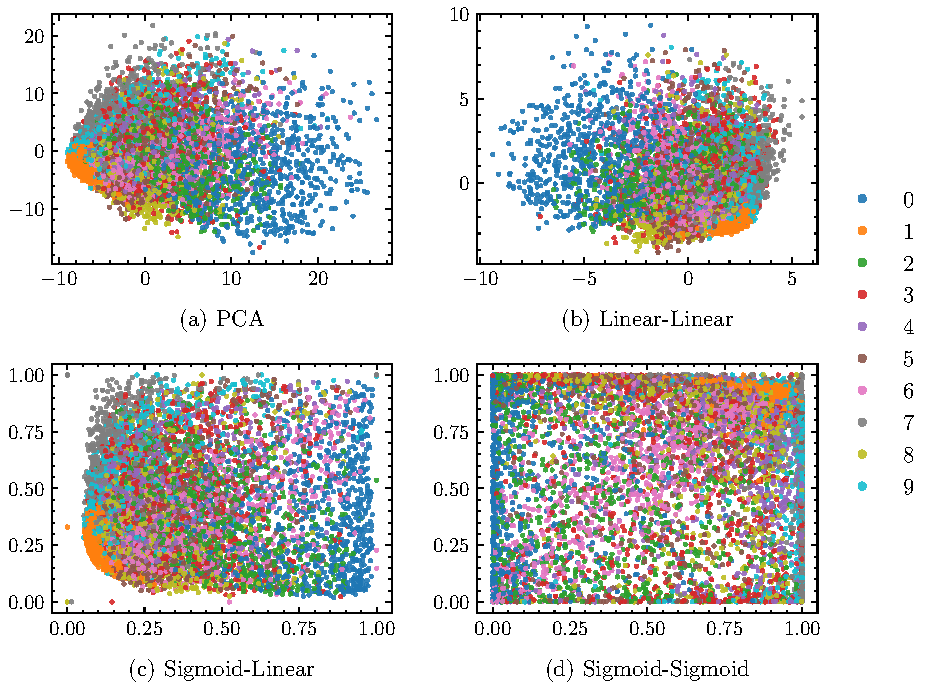
\includegraphics{autoencoders-nonlinearity.pdf}
	\caption[Latente Repräsentationen von PCA und drei Autoencoder mit unterschiedlichen Aktivierungsfunktionen]{Dargestellt sind die latenten Repräsentationen $\mat{Y}$ einer \captiona Principal Component Analysis und mehrerer Autoencoder mit \captionb linearen Aktivierungsfunktionen, \captionc Sigmoid-Aktivierung im Encoder und linearem Decoder und \captiond Sigmoid-Aktivierungen im Encoder und Decoder. Alle Autoencoder wurden mit \textit{weight decay} ($\lambda = \num{e-6}$) trainiert.}
	\label{fig:Autoencoder-Nichtlinearitaet}
\end{figure}
Als Referenz ist in \captiona die latente Repräsentation der Principal Component Analysis abgebildet. Wie bereits im theoretischen Zusammenhang erklärt, lernt ein linearer Autoencoder mit \textit{weight decay} die Richtungen der Hauptkomponenten bis hin zu einer orthogonalen Transformation. Vergleicht man \figref{fig:Autoencoder-Nichtlinearitaet} \captiona mit \captionb ist dies in der Tat der Fall. Ist der Encoder nichtlinear, so besteht immer noch eine große Ähnlichkeit zu der von PCA gefundenen latenten Repräsentation. Dies stimmt mit der von \textcite{Bourlard.1988} gemachten formalen Beobachtung überein. Ist der Decoder ebenfalls nichtlinear, so weicht die gefundene Repräsentation deutlich von der Repräsentation der Principal Component Analysis und anderer (teilweise) linearer Autoencoder ab. Bei der Hinzunahme von Nichtlinearität zum Autoencoder, gehen die beschriebenen Zusammenhänge also erst vollständig verloren, wenn sowohl Encoder als auch Decoder nichtlinear sind.
